\documentclass[a4paper]{article}

\usepackage{fullpage} % Package to use full page
\usepackage{parskip} % Package to tweak paragraph skipping
\usepackage{tikzsymbols}
\usepackage{tikz} % Package for drawing
\usepackage{amsmath}
\usepackage{hyperref}
\usepackage{float}
\makeatletter
\renewcommand{\@seccntformat}[1]{}
\makeatother
\usetikzlibrary{shapes.geometric}
\usetikzlibrary{decorations.pathreplacing}


\title{Understanding Acceleration vs. Time with Pendulums Day 2}
\author{Luke Bordonaro}
\date{}

\begin{document}

\maketitle

\section{Introduction}

Today we will discuss the data and graph that we recorded last class. We will attempt to understand why the acceleration vs. time graph is cyclic in nature, and use observations to estimate the acceleration due to gravity on Earth. 

\section{Materials}
\begin{itemize}
    \item An Android or Apple smart phone with the \textit{Science Journal} app installed
    \item String
    \item A plastic bag, large enough to hold your phone securely
    \item A wooden dowel
    \item A ruler/meter stick
\end{itemize}

\section{Setup}

\begin{enumerate}
    \item First, form \textit{groups of $3$} to work with.
    \item Next, insert a phone into a plastic bag. 
    \item Poke a hole through the plastic bag and tie one end of the string to the plastic bag through the hole.
    \item Tie the other end of the string around the center of your wooden dowel, such that the length of the string from the dowel to the phone is the desired length $l$.
    \item Position the dowel between two desks (or over the edge of only one desk). The setup should look like the figure below.
\end{enumerate}

\begin{figure}[H]
    \centering
    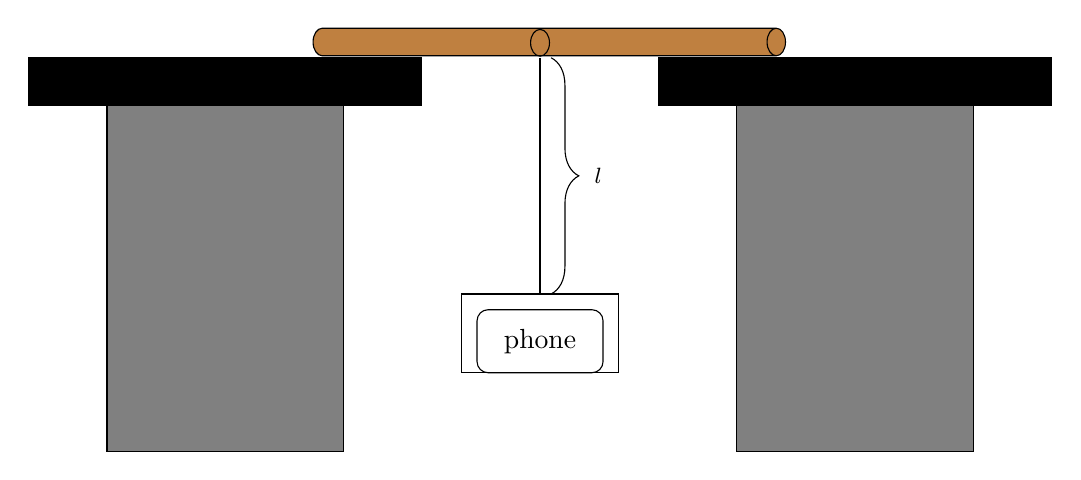
\begin{tikzpicture}[y=-1cm]
        \draw [fill=black] (0, 0) rectangle (5,0.6);
        \draw [fill=gray] (1, 0.6) rectangle (4, 5);
        \draw [fill=black] (8, 0) rectangle (13, 0.6);
        \draw [fill=gray] (9, 0.6) rectangle (12, 5);
        \node at (6.5, -0.2) [cylinder, draw, fill=brown, minimum height=60mm, minimum width=3.5mm] {};
        \draw (6.5, 0) -- (6.5, 3);
        \draw (6.5,-0.19) ellipse (.12 and .17);
        \draw [decorate,decoration={brace,amplitude=10pt},xshift=4pt,yshift=0pt]
(6.5,  0) -- (6.5, 3) node [black,midway,xshift=0.6cm] 
{\footnotesize $l$};
        \draw (5.5, 3) rectangle (7.5 ,4);
        \draw[rounded corners] (5.7, 3.2) rectangle (7.3 ,4) node[midway] {phone};
    \end{tikzpicture}
    \caption{The initial setup.}
\end{figure}

\section{Procedure}

After setting everything up as shown above, open the science journal app on the phone being used (you should be able to use the touch screen through the bag). Begin a new experiment and following the steps below to begin recording acceleration in the $x$ direction.

\begin{figure}[H]
    \centering
    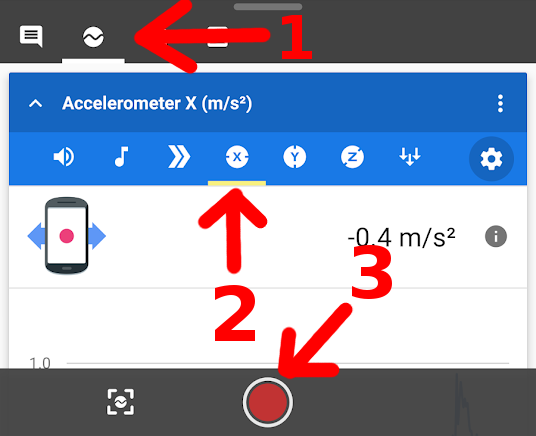
\includegraphics[scale=0.5]{start.png}
    \caption{How to start recording}
    \label{fig:my_label}
\end{figure}

Once you begin recording, lift the phone so that, when released, it will swing in an arc. Make sure you lift the phone so that the screen is pointing up.

\begin{figure}[H]
    \centering
    \begin{tikzpicture}[y=-1cm]
        \draw (0,0) circle (.2);
        \draw (-0.2, 0.1) -- (-3, 2);
        \draw[rotate around={-55:(-3,2)}] (-3.1, 2) rectangle (-2.9,4);
    \end{tikzpicture}
    \caption{How to begin the pendulum}
    \label{fig:my_label}
\end{figure}

Release the phone and let the pendulum oscillate several times. Afterwards, stop the recording and observe the recorded data. We are looking for something cyclic, such as 

\begin{figure}[H]
    \centering
    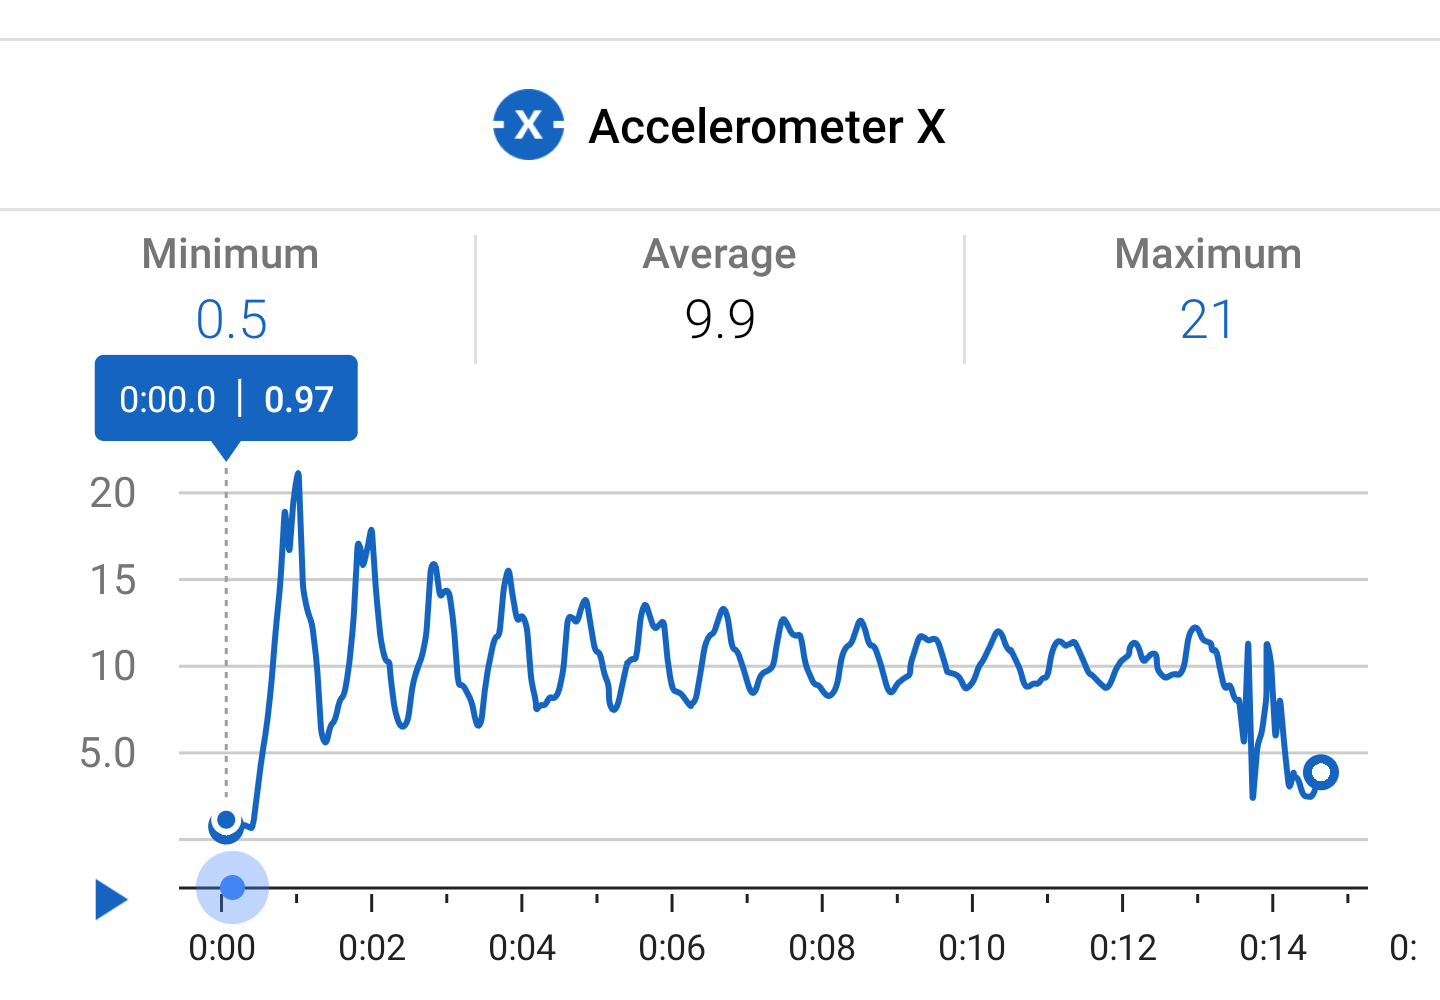
\includegraphics[scale=0.2]{graph.png}
    \caption{How to start recording}
    \label{fig:my_label}
\end{figure}

When you are done with your recordings, make sure to save the experiments on the \textit{Science Journal} app!

\section{Questions}

We will discuss these questions tomorrow $\dSmiley$. Make sure you do enough trials to think about the answers at home!

\begin{enumerate}
    \item When the phone is first released, is the acceleration at a \textit{maximum} or \textit{minimum}? Why?
    \item From the graph, calculate the period of the pendulum swing (how long it takes to complete one full cycle).
    \item Try releasing the phone from different starting angles; does the period change? Why or why not?
    \item Try recording velocity as a function of time. How does that graph compare with the acceleration graph?
\end{enumerate}

\section{Data}

Something we have control over is how long we make the string. Now that we understand the setup and procedure, go ahead and calculate the period of the pendulum with different lengths! What happens when the length is doubled? What happens when the length is multiplied by $4$? 

\begin{table}[H]
\renewcommand{\arraystretch}{3}
\centering
\begin{tabular}{|l@{\hspace{3em}}|l@{\hspace{2em}}|l@{\hspace{2em}}|l@{\hspace{2em}}|l@{\hspace{2em}}|}
\hline
length & trial $1$ period & trial period $2$ & trial period $3$ & average period \\ \hline
    &           &           &           &                \\ \hline
    &           &           &           &                \\ \hline
    &           &           &           &                \\ \hline
\end{tabular}
\end{table}

Make a plot of average period vs. length. What kind of relationship do you see?

\begin{figure}[H]
\centering
\begin{tikzpicture}
      \draw[->] (0,0) -- node[below] {$l$} (6,0);
      \draw[->] (0,0) -- node[left] {$T$} (0,6);
\end{tikzpicture}
\end{figure}


\end{document}